\documentclass[twoside]{article}


\usepackage[sc]{mathpazo} % Use the Palatino font
\usepackage[T1]{fontenc} % Use 8-bit encoding that has 256 glyphs
\linespread{1.3} % Line spacing - Palatino needs more space between lines
\usepackage{microtype} % Slightly tweak font spacing for aesthetics

\usepackage[hmarginratio=1:1,top=32mm,columnsep=20pt]{geometry} % Document margins
\usepackage{multicol} % Used for the two-column layout of the document
\usepackage[hang, small,labelfont=bf,up,textfont=it,up]{caption} % Custom captions under/above floats in tables or figures
\usepackage{booktabs} % Horizontal rules in tables
\usepackage{float} % Required for tables and figures in the multi-column environment - they need to be placed in specific locations with the [H] (e.g. \begin{table}[H])
\usepackage{hyperref} % For hyperlinks in the PDF

\usepackage{lettrine} % The lettrine is the first enlarged letter at the beginning of the text
\usepackage{paralist} % Used for the compactitem environment which makes bullet points with less space between them

\usepackage{titlesec} % Allows customization of titles
\renewcommand\thesection{\Roman{section}} % Roman numerals for the sections
\renewcommand\thesubsection{\Roman{subsection}} % Roman numerals for subsections
\titleformat{\section}[block]{\large\scshape\centering}{\thesection.}{1em}{} % Change the look of the section titles
\titleformat{\subsection}[block]{\large}{\thesubsection.}{1em}{} % Change the look of the section titles

\usepackage{fancyhdr} % Headers and footers
\pagestyle{fancy} % All pages have headers and footers
\fancyhead{} % Blank out the default header
\fancyfoot{} % Blank out the default footer
\fancyhead[C]{USC EE511} % Custom header text
\fancyfoot[RO,LE]{\thepage} % Custom footer text



\usepackage{multicol}
\usepackage{listings}
\usepackage{graphicx}
\usepackage{caption}
\usepackage{subcaption}
\usepackage{hyperref}
\usepackage{color}
\usepackage{float}
\usepackage{mathtools}
\usepackage{amssymb}
\usepackage{wrapfig}


\lstset{ %
language=Matlab,                % choose the language of the code
basicstyle=\footnotesize,       % the size of the fonts that are used for the code
numbers=left,                   % where to put the line-numbers
numberstyle=\footnotesize,      % the size of the fonts that are used for the line-numbers
stepnumber=1,                   % the step between two line-numbers. If it is 1 each line will be numbered
numbersep=5pt,                  % how far the line-numbers are from the code
backgroundcolor=\color{white},  % choose the background color. You must add \usepackage{color}
showspaces=false,               % show spaces adding particular underscores
showstringspaces=false,         % underline spaces within strings
showtabs=false,                 % show tabs within strings adding particular underscores
frame=single,           % adds a frame around the code
tabsize=2,          % sets default tabsize to 2 spaces
captionpos=b,           % sets the caption-position to bottom
breaklines=true,        % sets automatic line breaking
breakatwhitespace=false,    % sets if automatic breaks should only happen at whitespace
escapeinside={\%*}{*)}          % if you want to add a comment within your code
}
%----------------------------------------------------------------------------------------
%	TITLE SECTION
%----------------------------------------------------------------------------------------

\title{\vspace{-15mm}\fontsize{24pt}{10pt}\selectfont\textbf{Project \#6 - Continuous Sampling }} % Article title

\author{
\large
\textsc{Li Yicheng}\thanks{\href{https://github.com/IAMLYCHEE/EE511}{github link: https://github.com/IAMLYCHEE/EE511-PROJ6} }\\[2mm] % Your name
\normalsize USCID:7827077047\\
\normalsize email: l.y.c.liyicheng@gmail.com \\ % Your institution
\normalsize USC Viterbi of Engineering
\vspace{-5mm}
}

\date{}

%----------------------------------------------------------------------------------------

\begin{document}

\maketitle % Insert title

\thispagestyle{fancy} % All pages have headers and footers
% \begin{multicols*}{2}
\section{Generate Normal Random Variables}
\begin{multicols*}{2}
\subsection{\normalsize{Importance of Normal Distribution}}
 It has one of the important properties called central theorem. Central theorem means relationship between shape of population distribution and shape of sampling distribution of mean. This means that sampling distribution of mean approaches normal as sample size increase.In case the sample size is large the normal distribution serves as good approximation.Due to its mathematical properties it is more popular and easy to calculate.It is used in statistical quality control in setting up of control limits.The whole theory of sample tests t, f and chi-square test is based on the normal distribution.\\
\subsection{\normalsize{Box Muller method}}
\subsubsection{Mathematical principle}
\noindent \textbf {Basic Form}\\
Suppose U1 and U2 are independent random variables that are uniformly distributed in the interval (0, 1). Let\\
${\displaystyle Z_{0}=R\cos(\Theta )={\sqrt {-2\ln U_{1}}}\cos(2\pi U_{2})\,} $\\
and\\
${\displaystyle Z_{1}=R\sin(\Theta )={\sqrt {-2\ln U_{1}}}\sin(2\pi U_{2}).\,}$\\
Then $Z_0$ and $Z_1$ are independent random variables with a standard normal distribution.\\
Partial Proof:\\
${\displaystyle R^{2}=-2\cdot \ln U_{1}\,}$\\
and\\
$\because$
$\mathbb{P}(R^2 \leq x) = \mathbb{P}(-2lnU_1 \leq x)\\ =
\mathbb{P}(lnU_1 \geq -\frac{x}{2})\\
=\mathbb{P}(U_1 \geq e^{-\frac{x}{2}})\\
=1-e^{-\frac{x}{2}}$\\
therefore\\
pdf for $R^2$ is $\frac{1}{2}e^{-\frac{x}{2}}$ \\
$R^2$ is the square of the norm of the standard bivariate normal variable (X, Y), it has the chi-squared distribution with two degrees of freedom($R^2\sim \chi_2^2$),which also coincides with the exponential distribution.\\
\noindent \textbf {Rescale and Shift}\\
 To derive normal distribution X $\sim \displaystyle N(\mu,\sigma^2)$ from $N \sim \displaystyle N(0,1)$, we let $X = \sigma  N + \mu$\\ 
 Proof:\\
$\lim_{\delta \to 0}\mathbb{P}(x \leq N \leq x + \delta ) \\
= \delta \frac{1}{\sqrt{2\pi}}e^{-\frac{x^2}{2}}$\\
and  $X = \sigma  N + \mu$\\ 
$\lim_{\delta \to 0}\mathbb{P}(x \leq X \leq x + \delta )\\
=\lim_{\delta \to 0}\mathbb{P}(x \leq \sigma N + \mu \leq x + \delta )\\
=\lim_{\delta \to 0}\mathbb{P}(\frac{x-\mu}{\sigma} \leq N \leq \frac{x + \delta - \mu}{\sigma} )\\
=\delta \frac{1}{\sqrt{2\pi}\sigma}e^{- \frac{(x-\mu)^2}{2\sigma^2}}$\\
therefore: $X \sim N(\mu,\sigma^2)$\\
\subsubsection{Implementation}
 \begin{lstlisting}
 function [x,y,telapsed] = generateRandNBoxMuller(m1,v1,m2,v2,sampleAmount)
%generate two random variables using Box-Muller method
%input: 
%m1,m2: the expectation of the desired output normal distribution
%v1,v2: the variance of the desired output normal distribution
%sampleAmount: the amount of samples to generate 

tstart = tic;
u1 = rand(sampleAmount,1);
u2 = rand(sampleAmount,1);

% Generate X and Y that are N(0,1) random variables and independent
X = sqrt( - 2*log(u1)).*cos(2*pi*u2 ); 
Y = sqrt( - 2*log(u1)).*sin(2*pi*u2 );

% fit them to a random variable 
x = sqrt(v1)*X + m1; % x~ N(m1,v1)
y = sqrt(v2)*Y + m2; % y~ N(m2,v2)

telapsed = toc(tstart);
\end{lstlisting}

\subsubsection{Result}
\noindent \textbf {run the following script for simulation}\\
\begin{lstlisting}
%Box Muller sample method
[x,y,telapsed]=generateRandNBoxMuller(1,4,2,9,1000);
A = x + y;
covariance = cov(x,y);
figure
histogram(A,35,'BinLimits',[-15,15],'Normalization','probability');
hold on
t = -15 : 0.03 : 15;
theoPdf = theoreticalPdfNormal(3,13,t) ;
plot(t,theoPdf);
xlabel('value')
ylabel('probability')
title('Box Muller method (1000 sample)')
legend('Box Muller','Theoretical')
sampleMean = mean(A);
sampleVariance = var(A);
\end{lstlisting}
\begin{figure}[H]
   \centering
   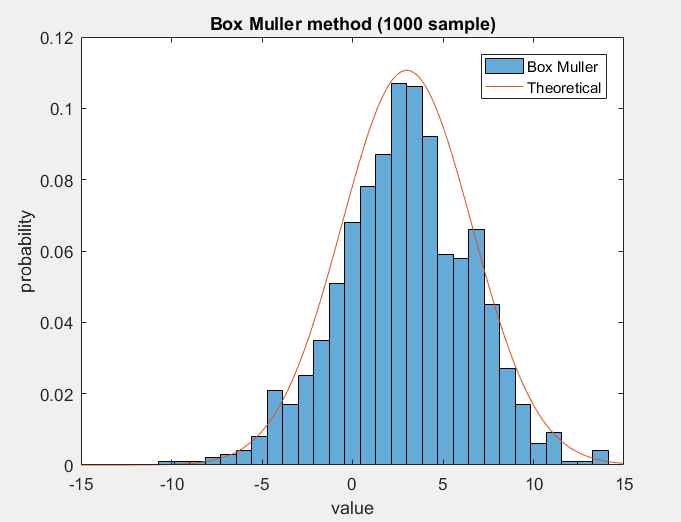
\includegraphics[width = 0.5\textwidth]{../data/solution1_1_1000.png}  
   \caption{Box Muller method 1000 sample}
\end{figure}
\noindent \textbf {data}:
\begin{figure}[H]
   \centering
   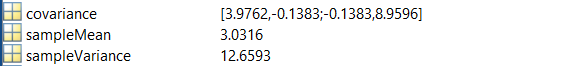
\includegraphics[width = 0.5\textwidth]{../data/solution1result.png}  
   \caption{data}
\end{figure}
from the data: we can observe the mean of the sample is 3.0316 and the variance is 12.6593. Moreover, from the covariance matrix, we can observe the X and Y's property. X has the variance of 3.9762 and Y has the variance of 8.9596, their covariance is -0.1383(near 0). Therefore, independent normal distribution $N(1,4)$ and $N(2,9)$ are sampled.  

\subsection{\normalsize{Polar Marsaglia Method}}
\subsubsection{Mathematical Principle}
\noindent \textbf {Basic Form}\\
Given u and v, independent and uniformly distributed in the closed interval [-1, +1], set s = R2 = u2 + v2. (Clearly ${\displaystyle \scriptstyle R={\sqrt {s}}})$  If s = 0 or s $\geq$ 1, discard u and v, and try another pair (u, v). Because u and v are uniformly distributed and because only points within the unit circle have been admitted, the values of s will be uniformly distributed in the open interval (0, 1), too. The latter can be seen by calculating the cumulative distribution function for s in the interval (0, 1). This is the area of a circle with radius ${\displaystyle \scriptstyle {\sqrt {s}}}$ , divided by ${\displaystyle \scriptstyle \pi }$ . From this we find the probability density function to have the constant value 1 on the interval (0, 1). Equally so, the angle θ divided by $2 \pi$ is uniformly distributed in the interval [0, 1) and independent of s.\\
\subsubsection{Implementation}
\begin{lstlisting}
function [x,y,telapsed]=generateRandnMarsaPolar(m1,v1,m2,v2,sampleAmount)
%generate two random variables using Marsaglia's polar method
%input: 
%m1,m2: the expectation of the desired output normal distribution
%v1,v2: the variance of the desired output normal distribution
%sampleAmount: the amount of samples to generate 
tstart = tic;
i = 0; % the random number generated by the algorithm 
% Geberate X and Y that are N(0,1) random variables and independent
while(i<=sampleAmount)
    u1 = 2*rand()-1;
    u2 = 2*rand()-1;
    s = u1^2 + u2^2;
    if(s < 1)
        i = i + 1;
        X(i) = sqrt(-2*log(s)/s)*u1;
        Y(i) = sqrt(-2*log(s)/s)*u2;
    end
end
% Scale them to a particular mean and variance 
x = sqrt(v1)*X + m1; % x~ N(M1,V1)
y = sqrt(v2)*Y + m2; % y~ N(M2,V2)
telapsed = toc(tstart);
\end{lstlisting}

\subsubsection{Result}
\noindent \textbf {run the following script to get 1000000 samples using Polar Marsaglia Method and compare the computational time required to generate 1000000 pairs of independent samples.}\\
\begin{lstlisting}
%Polar Marsaglia method
clear
[x,y,telapsed1]=generateRandnMarsaPolar(0,1,0,1,1000000);  
sampleMeanX = mean(x);
sampleMeanY = mean(y);
sampleVarianceX = var(x);
sampleVarianceY = var(y);
covariance = cov(x,y);
[x2,y2,telapsed2] = generateRandNBoxMuller(0,1,0,1,1000000);
\end{lstlisting}
\noindent \textbf {Data}\\
\begin{figure}[H]
   \centering
   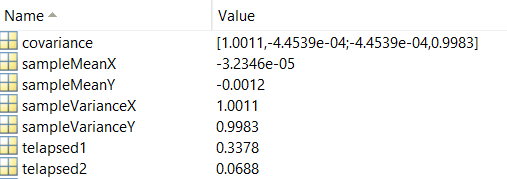
\includegraphics[width = 0.5\textwidth]{../data/solution1result2.png}  
   \caption{Data for 1000000 samples,Polar Marsaglia method}
\end{figure}
From the data, we can see X with a mean: -3.2346e-05 and Y with a mean: -0.0012, and X has variance of 1.0011, Y has variance of  0.9983. Therefore, X,Y fit normal distribution well. Moreover, they have the covariance of -4.4539e-04, that means they are very little correlated. \\
The time used with Box-Muller Method is 0.0688 while with Marsaglia Method is 0.3378. Box-Muller is more efficient because there is a selection process in Ploar Marsaglia method. \\

\section{Generate Gamma Random Variables}
\subsection{\normalsize{Accept-Reject Sampling}}
\noindent \textbf {(a):}Understanding the accept-reject method. The rejection sampling method generates sampling values from a target X with arbitrary probability density function f(x) by using a proposal distribution Y with probability density g(x). The idea is that one can generate a sample value from X by instead sampling from Y and accepting the sample from Y with probability ${\displaystyle f(x)/(Mg(x))}$, repeating the draws from Y until a value is accepted. \\
\noindent \textbf {(b):}First, we derive the constant M, M need to be make sure that $Mg(x) > f(x)$ should be true for every x, therefore, we take the max of $(f(x)/g(x))$ to determine the M. Then we using the accept-reject method to derive $f(x)$.\\
\underline{\emph{Algorithm:}}\\[10pt]
*1. Set random variable S which has distribution g(x)\\
*2. Compute the constant M\\
*3. Generate a sample s from S, generate a number u from std U[0,1]\\
*4. if u< p(s)/Mg(s) , accept and record s, else reject.\\
*5. Repeat 3,4 for trail\_budget times.\\

\subsection{\normalsize{Implementation}}
The exponential distribution with parameter 0.1 is used as my g(x), because it is easy to use inverse samoling method to generate a sample from exponential distribution.\\
\noindent \textbf {Sample from exponential distribution}\\
\begin{lstlisting}
function sample = generateExpDis(lambda)
%generateExpDis(lambda)
%generate a sample given exponential distribution
%input parameter: lambda
%using inverse transform sampling
p = rand(1,1)- 1.00e-10;
sample = log( 1- p) / (-lambda);
\end{lstlisting}
\noindent \textbf {generating Gamma(5.5,1) accept-reject method}\\
\begin{lstlisting}
M = 2;
amount = 0;
trial = 0;
while amount < 1000
    %generate a sample from EXP(0.1)
    y = generateExpDis(0.1);
    if rand(1) < exp5_5(y)/(M*0.1 * exp(-0.1 * y))
        amount = amount + 1;
        sample(amount) = y;
    end
    trial = trial + 1;
end
efficiency = 1000/trial;
histogram(sample',35,'BinLimits',[0,40],'Normalization','probability');
hold on
t = 0: 0.1: 40;
plot(t,exp5_5(t))
xlabel('x')
ylabel('probability')
legend('accept-reject','theoretical')
title('Gamma(5.5,1)')
\end{lstlisting}

\subsection{\normalsize{Result}}
\begin{figure}[H]
   \centering
   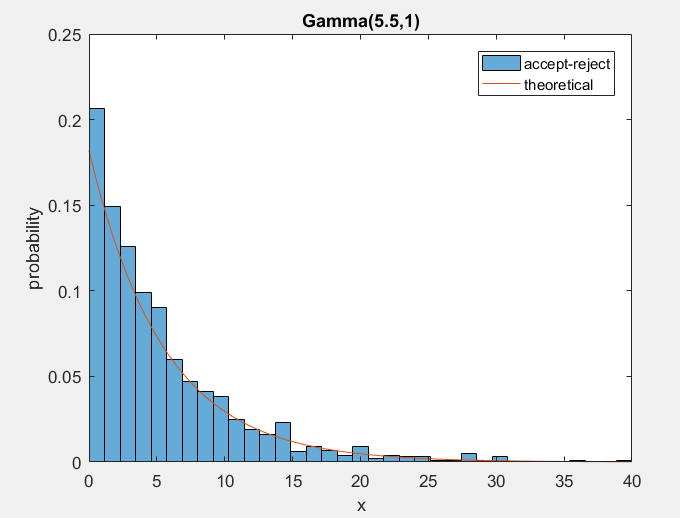
\includegraphics[width = 0.5\textwidth]{../data/gamma55.png}  
   \caption{Gamma(5.5,1)}
\end{figure}
\begin{figure}[H]
   \centering
   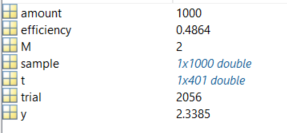
\includegraphics[width = 0.5\textwidth]{../data/datasolution2.png}  
   \caption{data}
\end{figure}
From the figure we can see the total trial is 2056, which means to generate 1000 samples we took 2056 trials, therefore, the acceptance rate is nearly every M sampling we get one sample.\\

\section{Alpha-Stable pdfs}
\subsection{\normalsize{Mathematic Principle}}
A random variable X is called stable if its characteristic function can be written as\\
${\displaystyle \varphi (\omega;\alpha ,\beta ,c,\mu )=\exp \left(i\omega\mu -|c\omega|^{\alpha }\left(1-i\beta \operatorname {sgn}(\omega)\Phi \right)\right)} $
${\displaystyle \Phi ={\begin{cases}\tan \left({\frac {\pi \alpha }{2}}\right)&\alpha \neq 1\\-{\frac {2}{\pi }}\log |\omega|&\alpha =1\end{cases}}}$\\
$\mu \in R$ is a shift parameter, $\beta \in [-1,1]$, called the skewness parameter, is a measure of asymmetry. Notice that in this context the usual skewness is not well defined, as for $\alpha < 2$the distribution does not admit 2nd or higher moments, and the usual skewness definition is the 3rd central moment.\\

\subsection{\normalsize{Implementation}}
\noindent \textbf {the codes are derived from github }{\href{https://github.com/markveillette/stbl}{github link: https://github.com/markvellette/stbl} }\\
Because it is a reference not the code written by myself, I just put it in the appendix.\\
\subsection{\normalsize{Result}}
\noindent \textbf {the following function is designed for one experiment}\\
\begin{lstlisting}
function experiment(alpha,beta,sampleAmount)
X = stblrnd(alpha,beta,1,0,sampleAmount,1);
histogram(X,'BinLimits',[-20,20],'Normalization','probability');
t = -20:0.2:20;
hold on
y = stblpdf(t,alpha,beta,1,0);
plot(t,y)
title(strcat('\alpha =', num2str(alpha) , '\beta =', num2str(beta)));
legend('histogram','theoretical')
hold off
%time series
figure
plot(X)
ylabel('sample value')
title(strcat('time series \alpha =', num2str(alpha) , '\beta =', num2str(beta)))
\end{lstlisting}
then run the following script to get all the figures and data:\\
\begin{lstlisting}
experiment(0.5,0,1000);
experiment(1,0,1000);
experiment(1.8,0,1000);
experiment(2.0,0,1000);
experiment(0.5,0.75,1000);
experiment(1.0,0.75,1000);
experiment(1.8,0.75,1000);
experiment(2.0,0.75,1000);
\end{lstlisting}
\noindent \textbf {Figures and Data}
\subsubsection{$\beta = 0$}
\begin{figure}[H]
   \centering
   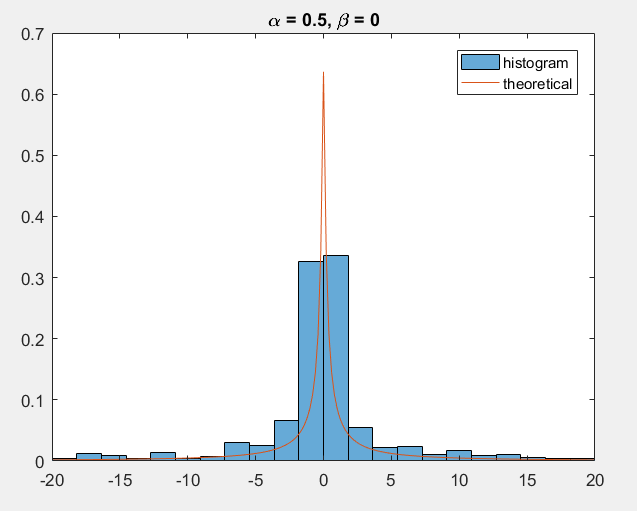
\includegraphics[width = 0.4\textwidth]{../data/a05b0.png}  
   \caption{$\alpha = 0.5, \beta = 0$}
\end{figure}
\begin{figure}[H]
   \centering
   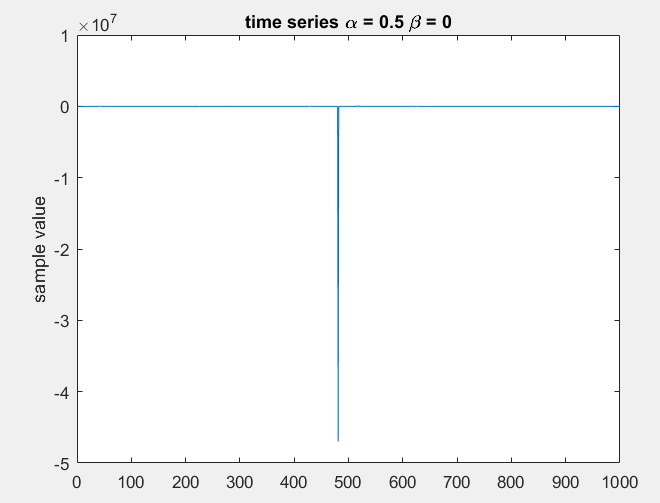
\includegraphics[width = 0.4\textwidth]{../data/a05b0time.png}  
   \caption{time series plot: $\alpha = 0.5, \beta = 0$}
\end{figure}

\begin{figure}[H]
   \centering
   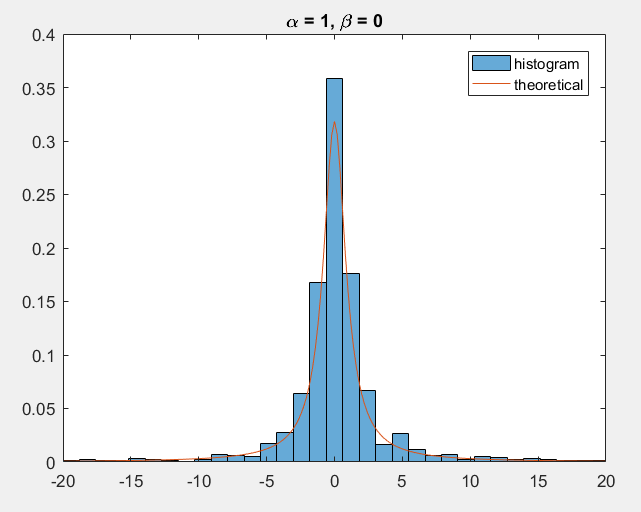
\includegraphics[width = 0.4\textwidth]{../data/a1b0.png}  
   \caption{$\alpha = 1.0, \beta = 0$}
\end{figure}
\begin{figure}[H]
   \centering
   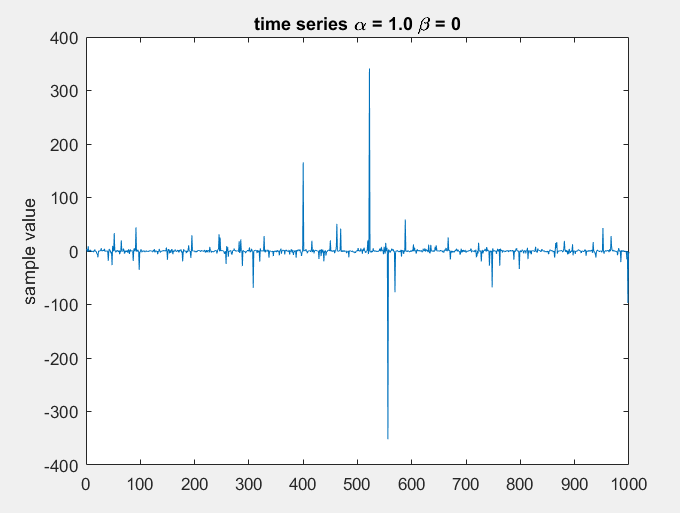
\includegraphics[width = 0.4\textwidth]{../data/a1b0time.png}  
   \caption{time series plot$\alpha = 1.0, \beta = 0$}
\end{figure}

\begin{figure}[H]
   \centering
   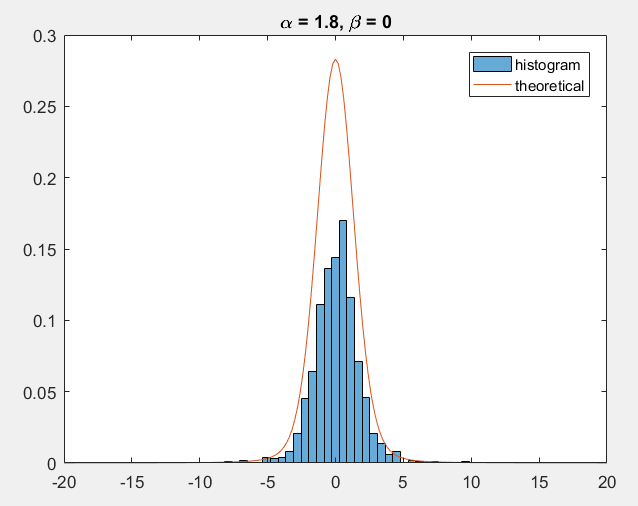
\includegraphics[width = 0.4\textwidth]{../data/a18b0.png}  
   \caption{$\alpha = 1.8, \beta = 0$}
\end{figure}
\begin{figure}[H]
   \centering
   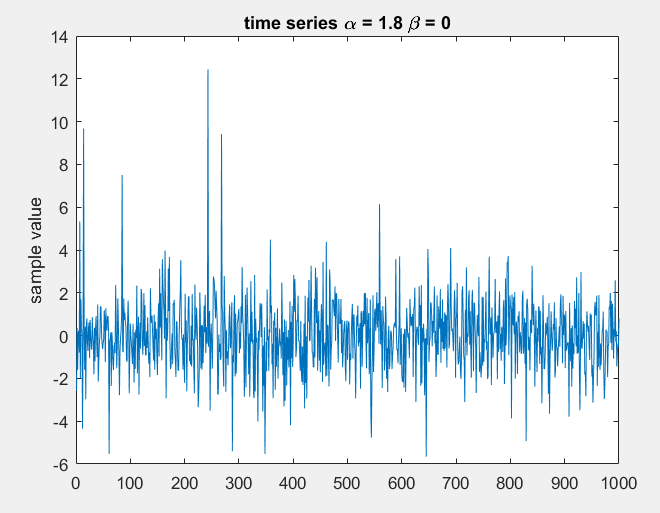
\includegraphics[width = 0.4\textwidth]{../data/a18b0time.png}  
   \caption{time series plot$\alpha = 1.8, \beta = 0$}
\end{figure}

\begin{figure}[H]
   \centering
   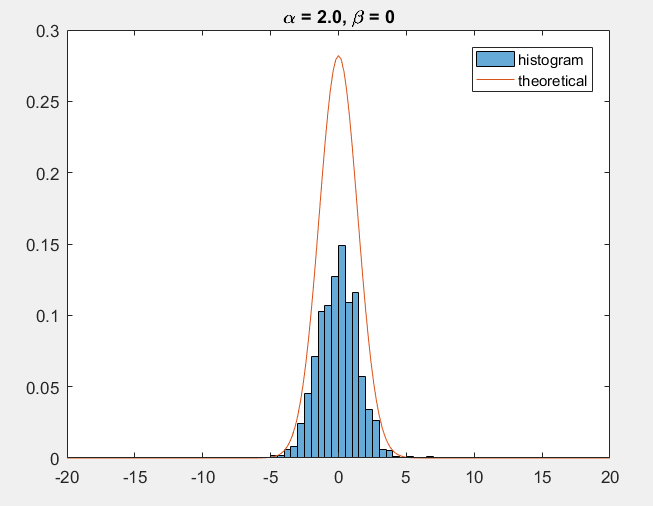
\includegraphics[width = 0.4\textwidth]{../data/a2b0.png}  
   \caption{$\alpha = 2.0, \beta = 0$}
\end{figure}
\begin{figure}[H]
   \centering
   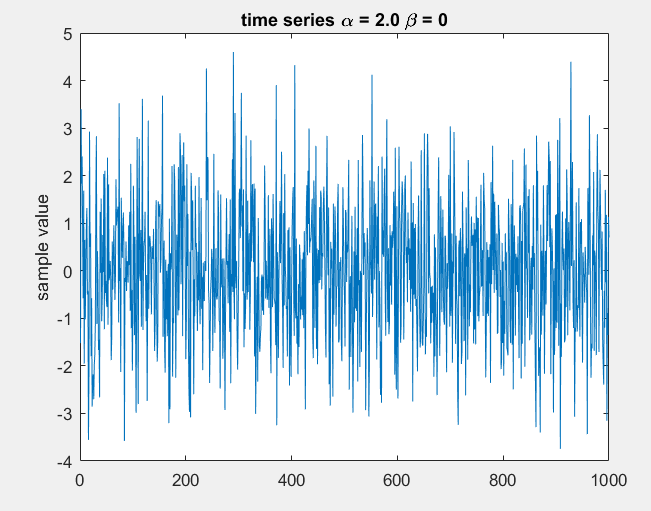
\includegraphics[width = 0.4\textwidth]{../data/a2b0time.png}  
   \caption{$time series plot\alpha = 2.0, \beta = 0$}
\end{figure}
From the figure it is clear that when alpha gets smaller, we got less oscillating, and the sample magnitude can be really large, when alpha becomes 2, we get the Gaussian distribution and the samples simulate the white noise.\\

\subsubsection{$\beta = 0.75$}
\begin{figure}[H]
   \centering
   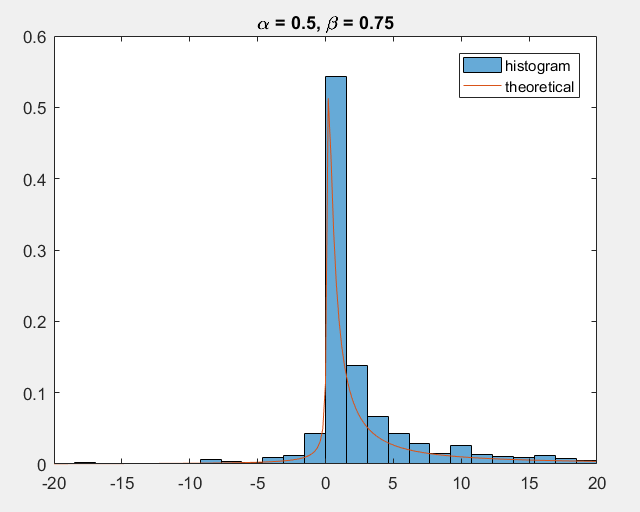
\includegraphics[width = 0.4\textwidth]{../data/a05b75.png}  
   \caption{$\alpha = 0.5, \beta = 0.75$}
\end{figure}
\begin{figure}[H]
   \centering
   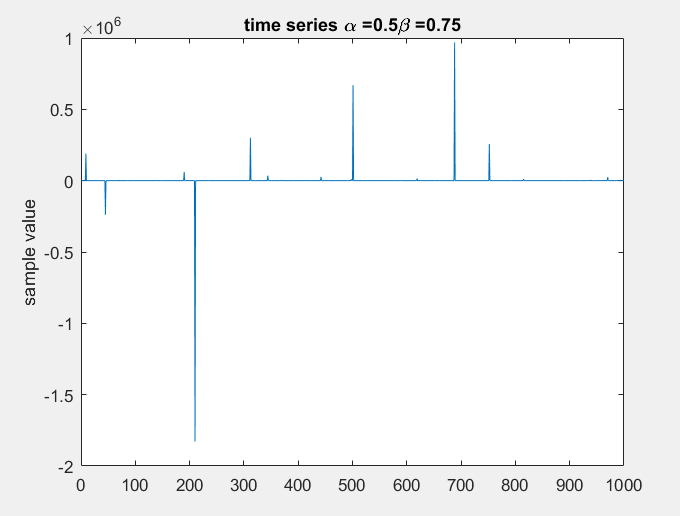
\includegraphics[width = 0.4\textwidth]{../data/a05b75time.png}  
   \caption{time series plot$\alpha = 0.5, \beta = 0.75$}
\end{figure}

\begin{figure}[H]
   \centering
   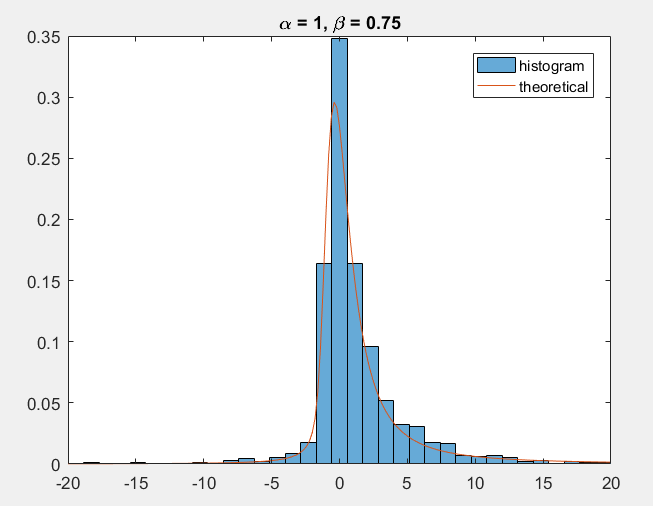
\includegraphics[width = 0.4\textwidth]{../data/a1b75.png}  
   \caption{$\alpha = 1.0, \beta = 0.75$}
\end{figure}
\begin{figure}[H]
   \centering
   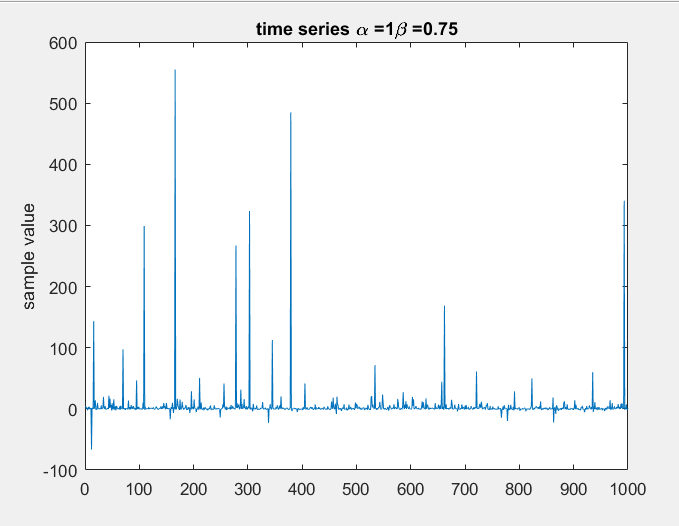
\includegraphics[width = 0.4\textwidth]{../data/a1b75time.png}  
   \caption{time series plot $\alpha = 1.0, \beta = 0.75$}
\end{figure}

\begin{figure}[H]
   \centering
   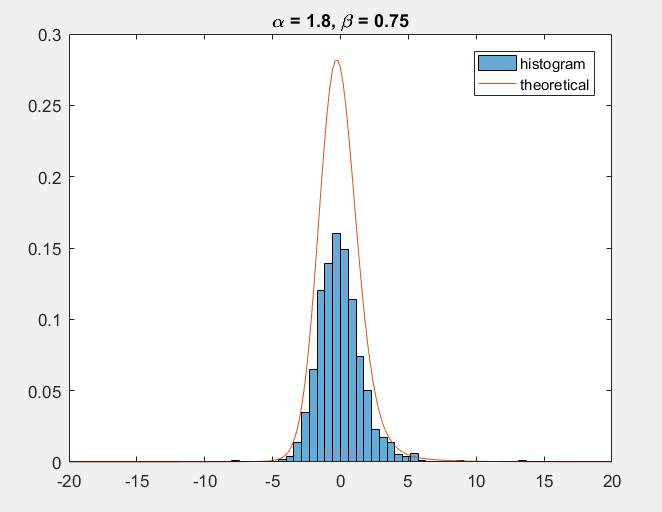
\includegraphics[width = 0.4\textwidth]{../data/a18b75.png}  
   \caption{$\alpha = 1.8, \beta = 0.75$}
\end{figure}
\begin{figure}[H]
   \centering
   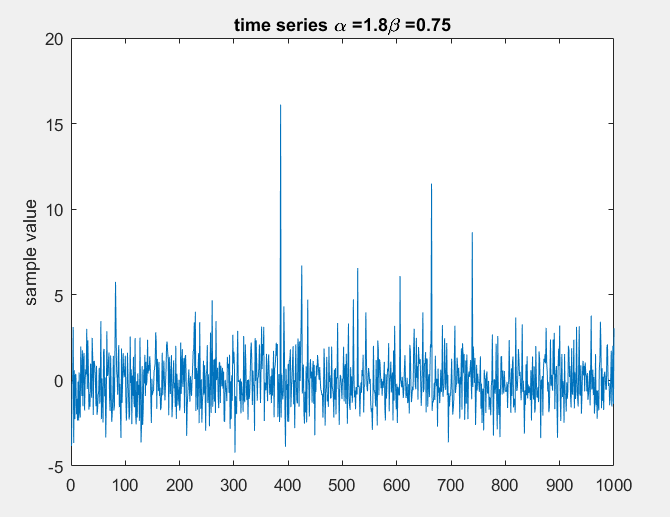
\includegraphics[width = 0.4\textwidth]{../data/a18b75time.png}  
   \caption{time series plot$\alpha = 1.8, \beta = 0.75$}
\end{figure}

\begin{figure}[H]
   \centering
   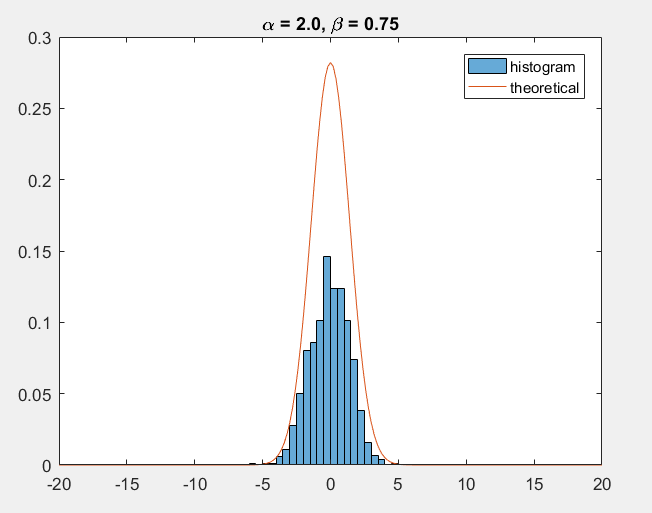
\includegraphics[width = 0.4\textwidth]{../data/a2b75.png}  
   \caption{$\alpha = 2.0, \beta = 0.75$}
\end{figure}
\begin{figure}[H]
   \centering
   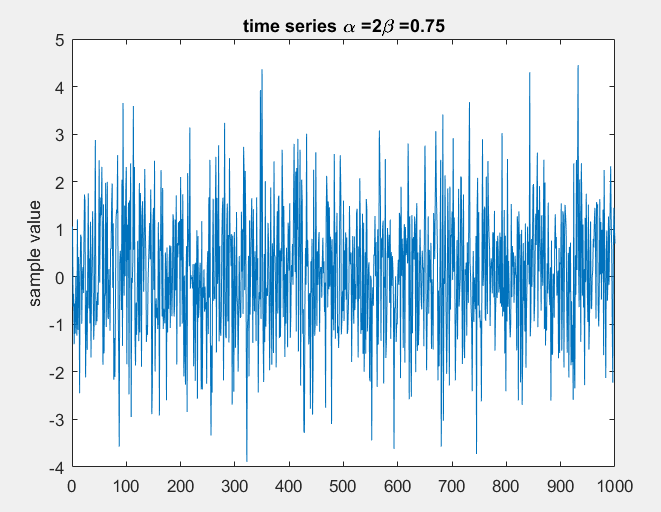
\includegraphics[width = 0.4\textwidth]{../data/a2b75time.png}  
   \caption{time series plot $\alpha = 2.0, \beta = 0.75$}
\end{figure}
From the figure, first it is obvious we can see a thick tail when $\alpha=0.5 ~and ~\alpha = 1.0$ because of the skewness. Also, it is clear that when alpha gets smaller, we got less oscillating, and the sample magnitude can be really large. Moreover, because of the change of skewness, it seems that the oscillation starts earlier.\\
\end{multicols*}

\section{Appendix}
\noindent \textbf {generate samples for Alpha-stable}
\begin{lstlisting}
function r = stblrnd(alpha,beta,gamma,delta,varargin)
%STBLRND alpha-stable random number generator.
% R = STBLRND(ALPHA,BETA,GAMMA,DELTA) draws a sample from the Levy 
% alpha-stable distribution with characteristic exponent ALPHA, 
% skewness BETA, scale parameter GAMMA and location parameter DELTA.
% ALPHA,BETA,GAMMA and DELTA must be scalars which fall in the following 
% ranges :
%    0 < ALPHA <= 2
%    -1 <= BETA <= 1  
%    0 < GAMMA < inf 
%    -inf < DELTA < inf
%
%
% R = STBLRND(ALPHA,BETA,GAMMA,DELTA,M,N,...) or 
% R = STBLRND(ALPHA,BETA,GAMMA,DELTA,[M,N,...]) returns an M-by-N-by-... 
% array.   
% 
%
% References:
% [1] J.M. Chambers, C.L. Mallows and B.W. Stuck (1976) 
%     "A Method for Simulating Stable Random Variables"  
%     JASA, Vol. 71, No. 354. pages 340-344  
%
% [2] Aleksander Weron and Rafal Weron (1995)
%     "Computer Simulation of Levy alpha-Stable Variables and Processes" 
%     Lec. Notes in Physics, 457, pages 379-392
%

if nargin < 4
    error('stats:stblrnd:TooFewInputs','Requires at least four input arguments.'); 
end

% Check parameters
if alpha <= 0 || alpha > 2 || ~isscalar(alpha)
    error('stats:stblrnd:BadInputs',' "alpha" must be a scalar which lies in the interval (0,2]');
end
if abs(beta) > 1 || ~isscalar(beta)
    error('stats:stblrnd:BadInputs',' "beta" must be a scalar which lies in the interval [-1,1]');
end
if gamma < 0 || ~isscalar(gamma)
    error('stats:stblrnd:BadInputs',' "gamma" must be a non-negative scalar');
end
if ~isscalar(delta)
    error('stats:stblrnd:BadInputs',' "delta" must be a scalar');
end


% Get output size
[err, sizeOut] = genOutsize(4,alpha,beta,gamma,delta,varargin{:});
if err > 0
    error('stats:stblrnd:InputSizeMismatch','Size information is inconsistent.');
end


%---Generate sample----

% See if parameters reduce to a special case, if so be quick, if not 
% perform general algorithm

if alpha == 2                  % Gaussian distribution 
    r = sqrt(2) * randn(sizeOut);

elseif alpha==1 && beta == 0   % Cauchy distribution
    r = tan( pi/2 * (2*rand(sizeOut) - 1) ); 

elseif alpha == .5 && abs(beta) == 1 % Levy distribution (a.k.a. Pearson V)
    r = beta ./ randn(sizeOut).^2;

elseif beta == 0                % Symmetric alpha-stable
    V = pi/2 * (2*rand(sizeOut) - 1); 
    W = -log(rand(sizeOut));          
    r = sin(alpha * V) ./ ( cos(V).^(1/alpha) ) .* ...
        ( cos( V.*(1-alpha) ) ./ W ).^( (1-alpha)/alpha ); 

elseif alpha ~= 1                % General case, alpha not 1
    V = pi/2 * (2*rand(sizeOut) - 1); 
    W = - log( rand(sizeOut) );       
    const = beta * tan(pi*alpha/2);
    B = atan( const );
    S = (1 + const * const).^(1/(2*alpha));
    r = S * sin( alpha*V + B ) ./ ( cos(V) ).^(1/alpha) .* ...
       ( cos( (1-alpha) * V - B ) ./ W ).^((1-alpha)/alpha);

else                             % General case, alpha = 1
    V = pi/2 * (2*rand(sizeOut) - 1); 
    W = - log( rand(sizeOut) );          
    piover2 = pi/2;
    sclshftV =  piover2 + beta * V ; 
    r = 1/piover2 * ( sclshftV .* tan(V) - ...
        beta * log( (piover2 * W .* cos(V) ) ./ sclshftV ) );      
          
end
    
% Scale and shift
if alpha ~= 1
   r = gamma * r + delta;
else
   r = gamma * r + (2/pi) * beta * gamma * log(gamma) + delta;  
end

end

\end{lstlisting}
\noindent \textbf {generate pdf for Alpha-Stable}
\begin{lstlisting}
function p = stblpdf(x,alpha,beta,gam,delta,varargin)
%P = STBLPDF(X,ALPHA,BETA,GAM,DELTA) returns the pdf of the stable 
% distribtuion with characteristic exponent ALPHA, skewness BETA, scale
% parameter GAM, and location parameter DELTA, at the values in X.  We use 
% the parameterization of stable distribtuions used in [2] - The 
% characteristic function phi(t) of a S(ALPHA,BETA,GAM,DELTA)
% random variable has the form
%
% phi(t) = exp(-GAM^ALPHA |t|^ALPHA [1 - i BETA (tan(pi ALPHA/2) sign(t)]
%                  + i DELTA t )  if alpha ~= 1
%
% phi(t) = exp(-GAM |t| [ 1 + i BETA (2/pi) (sign(t)) log|t|] + i DELTA t
%                                 if alpha = 1
%
% The size of P is the size of X.  ALPHA,BETA,GAM and DELTA must be scalars
% 
%P = STBLPDF(X,ALPHA,BETA,GAM,DELTA,TOL) computes the pdf to within an
% absolute error of TOL.
%
% The algorithm works by computing the numerical integrals in Theorem
% 1 in [1] using MATLAB's QUADV function.  The integrands  
% are smooth non-negative functions, but for certain parameter values 
% can have sharp peaks which might be missed.  To avoid this, STBLEPDF
% locates the maximum of this integrand and breaks the integral into two
% pieces centered around this maximum (this is exactly the idea suggested
% in [1] ).  
%
% If abs(ALPHA - 1) < 1e-5,  ALPHA is rounded to 1.
%
%P = STBLPDF(...,'quick') skips the step of locating the peak in the 
% integrand, and thus is faster, but is less accurate deep into the tails
% of the pdf.  This option is useful for plotting.  In place of 'quick',
% STBLPDF also excepts a logical true or false (for quick or not quick)
%
% See also: STBLRND, STBLCDF, STBLINV, STBLFIT
%
% References:
%
% [1] J. P. Nolan (1997)
%     "Numerical Calculation of Stable Densities and Distribution
%     Functions"  Commun. Statist. - Stochastic Modles, 13(4), 759-774
%
% [2] G Samorodnitsky, MS Taqqu (1994)
%     "Stable non-Gaussian random processes: stochastic models with 
%      infinite variance"  CRC Press
%

if nargin < 5
    error('stblpdf:TooFewInputs','Requires at least five input arguments.'); 
end

% Check parameters
if alpha <= 0 || alpha > 2 || ~isscalar(alpha)
    error('stblpdf:BadInputs',' "alpha" must be a scalar which lies in the interval (0,2]');
end
if abs(beta) > 1 || ~isscalar(beta)
    error('stblpdf:BadInputs',' "beta" must be a scalar which lies in the interval [-1,1]');
end
if gam < 0 || ~isscalar(gam)
    error('stblpdf:BadInputs',' "gam" must be a non-negative scalar');
end
if ~isscalar(delta)
    error('stblpdf:BadInputs',' "delta" must be a scalar');
end

% Warn if alpha is very close to 1 or 0
if ( 1e-5 < abs(1 - alpha) && abs(1 - alpha) < .02) || alpha < .02 
    warning('stblpdf:ScaryAlpha',...
        'Difficult to approximate pdf for alpha close to 0 or 1')
end

% warnings will happen during call to QUADV, and it's okay
warning('off');

% Check and initialize additional inputs
quick = false;
tol = [];
for i=1:length(varargin)
    if strcmp(varargin{i},'quick')
        quick = true;
    elseif islogical(varargin{i})
        quick = varargin{end};
    elseif isscalar(varargin{i})
        tol = varargin{i};
    end
end

if isempty(tol)
    if quick 
        tol = 1e-8;
    else
        tol = 1e-12;
    end
end
        

%======== Compute pdf ==========%

% Check to see if you are in a simple case, if so be quick, if not do
% general algorithm
if alpha == 2                  % Gaussian distribution 
    x = (x - delta)/gam;                 % Standardize
    p = 1/sqrt(4*pi) * exp( -.25 * x.^2 ); % ~ N(0,2)
    p = p/gam; %rescale

elseif alpha==1 && beta == 0   % Cauchy distribution
    x = (x - delta)/gam;              % Standardize
    p = (1/pi) * 1./(1 + x.^2); 
    p = p/gam; %rescale

elseif alpha == .5 && abs(beta) == 1 % Levy distribution 
    x = (x - delta)/gam;              % Standardize
    p = zeros(size(x));
    if  beta ==1
        p( x <= 0 ) = 0;
        p( x > 0 ) = sqrt(1/(2*pi)) * exp(-.5./x(x>0)) ./...
                                                x(x>0).^1.5;
    else
        p(x >= 0) = 0;
        p(x < 0 ) = sqrt(1/(2*pi)) * exp(.5./x(x<0)  ) ./...
                                            ( -x(x<0) ).^1.5;
    end
    p = p/gam; %rescale
    
elseif abs(alpha - 1) > 1e-5          % Gen. Case, alpha ~= 1
    
    xold = x; % Save for later
    % Standardize in (M) parameterization ( See equation (2) in [1] ) 
    x = (x - delta)/gam - beta * tan(alpha*pi/2);  
    
    % Compute pdf
    p = zeros(size(x));
    zeta = - beta * tan(pi*alpha/2);  
    theta0 = (1/alpha) * atan(beta*tan(pi*alpha/2));
    A1 = alpha*theta0;
    A2 = cos(A1)^(1/(alpha-1));
    exp1 = alpha/(alpha-1);
    alpham1 = alpha - 1;
    c2 = alpha ./ (pi * abs(alpha - 1) * ( x(x>zeta) - zeta) ); 
    V = @(theta) A2 * ( cos(theta) ./ sin( alpha*(theta + theta0) ) ).^exp1.*...
        cos( A1 + alpham1*theta ) ./ cos(theta);
    
    
    % x > zeta, calculate integral using QUADV
    if any(x(:) > zeta)
        xshift = (x(x>zeta) - zeta) .^ exp1;
        
        if beta == -1 && alpha < 1
            p(x > zeta) = 0;
        elseif ~quick % Locate peak in integrand and split up integral        
            g = @(theta) xshift(:) .* V(theta) - 1;
            R = repmat([-theta0, pi/2 ],numel(xshift),1);
            if abs(beta) < 1
                theta2 = bisectionSolver(g,R,alpha);
            else
                theta2 = bisectionSolver(g,R,alpha,beta,xshift);
            end
            theta2 = reshape(theta2,size(xshift));
            % change variables so the two integrals go from 
            % 0 to 1/2 and 1/2 to 1.
            theta2shift1 = 2*(theta2 + theta0);
            theta2shift2 = 2*(pi/2 - theta2);
            g1 = @(theta)  xshift .* ...
                V(theta2shift1 * theta - theta0);
            g2 = @(theta)  xshift .* ...
                V(theta2shift2 * (theta - .5) + theta2);
            zexpz = @(z) max(0,z .* exp(-z)); % use max incase of NaN
           
            p(x > zeta) = c2 .* ...
                (theta2shift1 .* quadv(@(theta) zexpz( g1(theta) ),...
                                        0 , .5, tol) ...
               + theta2shift2 .* quadv(@(theta) zexpz( g2(theta) ),...
                                       .5 , 1, tol) );                       
                              
        else  % be quick - calculate integral without locating peak
              % Use a default tolerance of 1e-6
            g = @(theta) xshift * V(theta);
            zexpz = @(z) max(0,z .* exp(-z)); % use max incase of NaN
            p( x > zeta ) = c2 .* quadv(@(theta) zexpz( g(theta) ),...
                                        -theta0 , pi/2, tol );  
        end
        p(x > zeta) = p(x>zeta)/gam; %rescale
        
    end
    
    % x = zeta, this is easy
    if any( abs(x(:) - zeta) < 1e-8 )  
        p( abs(x - zeta) < 1e-8 ) = max(0,gamma(1 + 1/alpha)*...
            cos(theta0)/(pi*(1 + zeta^2)^(1/(2*alpha))));
        p( abs(x - zeta) < 1e-8 ) = p( abs(x - zeta) < 1e-8 )/gam; %rescale
        
    end
   
    % x < zeta, recall function with -xold, -beta, -delta 
    % This doesn't need to be rescaled.
    if any(x(:) < zeta)
        p( x < zeta ) = stblpdf( -xold( x<zeta ),alpha,-beta,...
                        gam , -delta , tol , quick); 
    end
        
else                    % Gen case, alpha = 1
    
    x = (x - (2/pi) * beta * gam * log(gam) - delta)/gam; % Standardize
    
    % Compute pdf
    piover2 = pi/2;
    twooverpi = 2/pi;
    oneoverb = 1/beta;
    theta0 = piover2;
    % Use logs to avoid overflow/underflow
    logV = @(theta) log(twooverpi * ((piover2 + beta *theta)./cos(theta))) + ...
                 ( oneoverb * (piover2 + beta *theta) .* tan(theta) );
    c2 = 1/(2*abs(beta));
    xterm = ( -pi*x/(2*beta));
    
    if ~quick  % Locate peak in integrand and split up integral
             % Use a default tolerance of 1e-12
        logg = @(theta) xterm(:) + logV(theta) ;
        R = repmat([-theta0, pi/2 ],numel(xterm),1);
        theta2 = bisectionSolver(logg,R,1-beta);     
        theta2 = reshape(theta2,size(xterm));
        % change variables so the two integrals go from 
        % 0 to 1/2 and 1/2 to 1.
        theta2shift1 = 2*(theta2 + theta0);
        theta2shift2 = 2*(pi/2 - theta2);
        logg1 = @(theta)  xterm + ...
            logV(theta2shift1 * theta - theta0);
        logg2 = @(theta)  xterm + ...
            logV(theta2shift2 * (theta - .5) + theta2);
        zexpz = @(z) max(0,exp(z) .* exp(-exp(z))); % use max incase of NaN

        p = c2 .* ...
            (theta2shift1 .* quadv(@(theta) zexpz( logg1(theta) ),...
                                    0 , .5, tol) ...
           + theta2shift2 .* quadv(@(theta) zexpz( logg2(theta) ),...
                                   .5 , 1, tol) );     
      
       
    else % be quick - calculate integral without locating peak
              % Use a default tolerance of 1e-6
        logg = @(theta) xterm + logV(theta);
        zexpz = @(z) max(0,exp(z) .* exp(-exp(z))); % use max incase of NaN
        p = c2 .* quadv(@(theta) zexpz( logg(theta) ),-theta0 , pi/2, tol );
            
    end
    
    p = p/gam; %rescale
    
end

p = real(p); % just in case a small imaginary piece crept in 
             % This might happen when (x - zeta) is really small   

end




function X = bisectionSolver(f,R,alpha,varargin)
% Solves equation g(theta) - 1 = 0 in STBLPDF using a vectorized bisection 
% method and a tolerance of 1e-5.  The solution to this
% equation is used to increase accuracy in the calculation of a numerical
% integral.   
%
% If alpha ~= 1 and 0 <= beta < 1, the equation always has a solution
%
% If alpha > 1 and beta <= 1, then g is monotone decreasing
% 
% If alpha < 1 and beta < 1, then g is monotone increasing
%
% If alpha = 1,  g is monotone increasing if beta > 0 and monotone 
% decreasing is beta < 0.  Input alpha = 1 - beta to get desired results.
%
%


if nargin < 2
    error('bisectionSolver:TooFewInputs','Requires at least two input arguments.'); 
end

noSolution = false(size(R,1));
% if ~isempty(varargin)
%     beta = varargin{1};
%     xshift = varargin{2};
%     if abs(beta) == 1
%         V0=(1/alpha)^(alpha/(alpha-1))*(1-alpha)*cos(alpha*pi/2)*xshift;
%         if alpha > 1
%             noSolution = V0 - 1 %>= 0;
%         elseif alpha < 1
%             noSolution = V0 - 1 %<= 0;
%         end
%     end 
% end
    
tol = 1e-6;
maxiter = 30;
    
[N M] = size(R);
if M ~= 2
    error('bisectionSolver:BadInput',...
        '"R" must have 2 columns');
end

a = R(:,1);
b = R(:,2);
X = (a+b)/2;

try
    val = f(X);
catch ME
    error('bisectionSolver:BadInput',...
        'Input function inconsistint with rectangle dimension')
end
  
if size(val,1) ~= N
    error('bisectionSolver:BadInput',...
        'Output of function must be a column vector with dimension of input');
end

% Main loop
val = inf;
iter = 0;

while( max(abs(val)) > tol && iter < maxiter )
    X = (a + b)/2;
    val = f(X);
    l = (val > 0);
    if alpha > 1
        l = 1-l;
    end
    a = a.*l + X.*(1-l);
    b = X.*l + b.*(1-l);
    iter = iter + 1;
end



if any(noSolution(:))
    X(noSolution) = (R(1,1) + R(1,2))/2;
end

end

\end{lstlisting}


\end{document}